\documentclass[twocolumn]{article}
\usepackage[a4paper,margin=1in]{geometry}  % Adjust as needed
\usepackage{graphicx}
% \begin{figure*}
%     \centering
%     \includegraphics[width=\textwidth]{example-image}
%     \caption{A figure spanning both columns.}
%     \label{fig:example}
% \end{figure*}
\usepackage{lipsum}  % For placeholder text
\usepackage{microtype}  % Better text spacing
\usepackage{acronym}
\usepackage{hyperref}
\usepackage[utf8]{inputenc}
\usepackage{cleveref}
\usepackage[inline]{enumitem}
\usepackage[backend=bibtex,style=alphabetic]{biblatex}
\addbibresource{references.bib}

\title{
\LARGE{\textbf{Laboratory Activities Report}}
\\[2ex] \textit{Intelligent Robotic Systems} - A.Y. 2024/2025
}
\date{March 2025}
\author{Stefano Furi - \texttt{stefano.furi@studio.unibo.it} - 0001125057}

\begin{document}

\maketitle

%!TEX root = ../main.tex
\section{Lab Activity 1}

%!TEX root = ../main.tex
\section{Lab Activity 2}
The task goal is a composite behaviour from the behaviours developed in the
previous lab (see \Cref{sec:lab01}). Some differences can be highlighted in
terms of constraints: here, the robot:
\begin{itemize}
    \item must reach the light as fast as possibile;
    \item once reached the light, it should stay close to it;
    \item wheel velocities cannot exceed $15^{-2}m/s$.
\end{itemize}
For the second constraint, the implementation provided in the first lab
activity already satisfies it. The robot goes towards the light, and when
passing it, the highest intensity will be in back sensors, causing the robot to
subsequently turn 180 degrees, repeating this process infinitely. When it comes
to the third constraint, wheel velocities had already an upper bound in the
previous implementation. Lastly, in order to satisfy the first constraint we
need first to find a way to integrate the collision avoidance behaviour with
phototaxis.

\subsection{Behaviours Integration} In order to integrate behaviours, a sort of
``prioritisation'' is needed, both for fusing and arbitration techniques. In
order to keep the controller as simple as possibile, an arbitration behaviour
coordination schema is implemented. In this case, at each step a behaviour
among all possibile behaviours is selected. In this particular task, we
prioritise collision avoidance with respect to phototaxis. We firstly check the
presence of obstacles and if some are found, we steer the robot away from the
obstacles. Otherwise, we keep following the light. In this way light reaching
can be slowed down by the collision avoidance task, but for real world
scenarios high prioritisation collision avoidance could be strongly desirable.

\subsection{Behaviours Design} It is way more easier to design behaviours
independently and separately instead of creating a composite behaviour from
scratch. Even if composing behaviour could be challenging, we have various ways
to archive this, for example by means of the subabsumption architecture,
cooperative schemes, competitive schemes, etc. In this task's case in
particular, having already defined behaviours in the previous lab activity made
this one more focused on how to integrate them archive the desired behaviour
with the given constraints.

\subsubsection{Collision Avoidance}
When it comes to the collision avoidance task, the same implementation is
provided as the one for the first lab activity. Briefly: the robot retrieves
the maximum proximity sensor's value through a neighbour-weighted average. If
the maximum value is higher that a threshold (0.55), based on the angle of the
sensor the robot steers left or right.

When it comes to behaviours coordination, this behaviour could benefit a memory
mechanism. In order to be more efficient for accomplishing task goals, instead
of going the opposite way of the obstacle, the robot could choose a free
direction that favours the task of phototaxis. This is especially true for all
cases where there is the presence of tall obstacles that blocks the light
source. If we can keep a reference to where the light was lastly located, we
could prefer directions that helps the robot going towards the light faster
when avoiding obstacles (or circumnavigating them).

\subsubsection{Phototaxis}
As per the collision avoidance behaviour, the phototaxis one is implemented as
the previous lab activity but with some key difference in order to make the
robot reach the light in the fastest way as possible, and in order to reduce
the chances of collision when steering towards the light. Firstly, when
detecting the light in front (i.e. max light value is detected from sensors 1
or the $24^{th}$), we set wheel velocities to max speed in order to reach light
faster. On the other hand, when light is detected on every other sensors, we
perform a left or right steering keeping the opposite wheel velocity to the max
value and the other to zero, reducing the turn radius with respect to the first
lab activity implementation. In this way, we can reduce possibile impacts with
obstacles when performing a turn in order to go towards the light.


\subsection{Tests}
The overall behaviour performs well even under challenging arena/robot
configuration, for example having a noise of 0.05 on senors, having various
kind of obstacles inside the arena, especially tall obstacles that blocks
light. Other tests also involves more that one robot. In this case, robots
successfully avoid collisions with themselves, and wander under the light oncIe
reaching it, while avoiding collision with themselves.

%!TEX root = ../main.tex
\section{Lab Activity 3}

This laboratory assignment requires to implement a robot that performs
phototaxis while avoiding collisions with obstacles. Once reached the black
spot under the light, it should halt. This set of behaviours should be
implemented by means of a \textbf{subsumption architecture}. A set of
``competences'' should then be defined, and place them in a hierarchical,
layered architecture.

\subsection{Designing the Subsumption Architecture}\label{ssec:subsum}

The subsumption architecture is shown in \Cref{fig:sub-arch}. The layers are
placed in way that, when control is taken by an upper layer, it inhibits every
other underlying layer. Each layer can then use lower layers in order to
communicate or use the latter's information in order to implement higher-level
behaviours.
The \emph{competences} developed are the following (listed from lower to higher level):
%
\begin{figure}[ht]
    \centering
    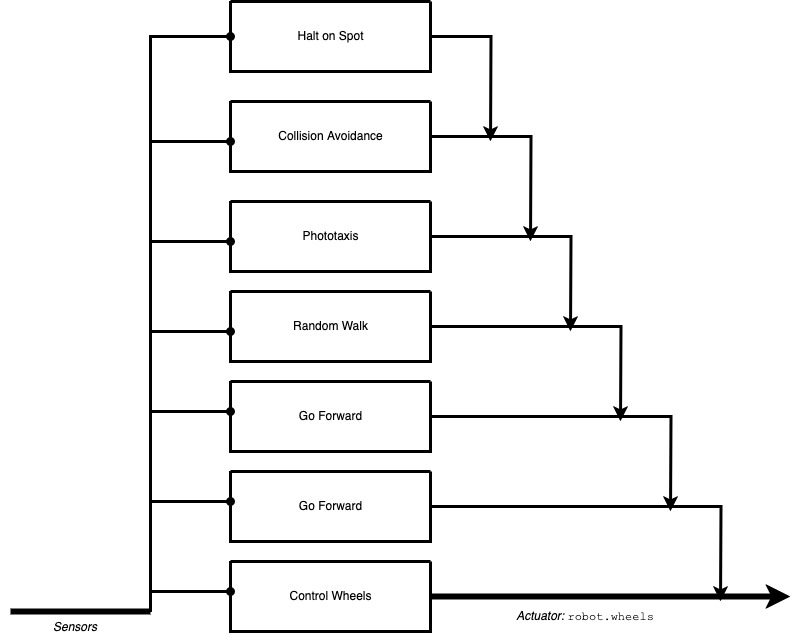
\includegraphics[width=0.6\textwidth]{figures/sub-arch.jpg}
    \caption{The Subsumption Architecture for archiving phototaxis while
        avoiding collisions and halting when under the light and over the black
        spot.}
    \label{fig:sub-arch}
\end{figure}
%
\begin{enumerate}
    \item \emph{Control Wheels} lets the definition of the simplest behaviour
        in order to control robot's wheels. It accepts a left and right
        velocities and sets the wheel velocities accordingly. It also avoid
        that the max speed of robot's wheels doesn't exceed $15^{-2}m/s$.
    \item \emph{Go Forward} defines a simple competence for moving forward,
        making use of its lower layer.
    \item \emph{Turn} accepts a direction on which the robot should turn to.
        Left or right turns are performed by multiplying current opposite wheel
        velocity by a factor (\texttt{TURN\_RATIO=3}) and the other wheel velocity by zero.
        This will let the robot to turn more gradually for finer turns.
    \item \emph{Random Walk} this competence performs a sub-optimal random walk by changing
        every $n$ steps robot wheels velocities randomly chosen.
    \item \emph{Follow Light}: phototaxis implementation. It picks maximum
        light value detected from sensors with the usual neighbour weighted
        average, and chose the direction to turn to based on which sensor
        yielded the maximum value.
    \item \emph{Avoid Front Obstacles}: collision avoidance implementation,
        with a difference that only front sensors are used for detecting
        collisions. If obstacles are detected, the controller checks collision
        for left, right and down, in this order. The first of these directions
        that does not contain an obstacle is used to perform a turn.
    \item \emph{Halt on Stop}: leveraging ground sensors, if any of those four
        detects that the robot is on the black spot, wheel velocities are set
        to zero.
\end{enumerate}
Having defined each layer and their dependencies, in order to keep the
``centralised'' piece of code as simple as possible, every layer makes use of a
shared boolean variable named \texttt{CONTROL\_TAKEN} which is reset at each
step. All layer includes the necessary checks for the shared variable before
performing their task. If they can take control, they set the variable to true,
if not, they early return.

With this approach we can archive coordination without complicating too much
the code, while keeping in mind that global state/variables can lead to
potential bugs and are sometimes discouraged. Another consideration that can be
made with shared variables in a distributed architecture like the subsumption
architecture, is that this can lead to race conditions, which can be easily
mitigated by means of mutex variables or atomic primitives (in this case an
atomic boolean).

\bigskip
With this approach, the control flow executes each layer in a top down fashion,
from the higher level to the lowest, and thanks to the shared state there is no
need of centralised coordination or inhibition by the main control flow.

%!TEX root = ../main.tex
\section{Lab Activity 4}
This lab assignment requires the usage of a \textbf{motor schema} in order to
implement a behaviour-based control for the task of phototaxis, while avoiding
collisions with other objects. The constraints are about maximum wheels
velocities ($15^{-2}m/s$) and that the robot must reach the light source as
fast as possible.

\subsection{Motor Schema Design}
First thing first, we define the potential fields that characterise the environment:
\begin{itemize}
	\item An \emph{attractive} potential field is applied to the light source,
	      with a variation that resembles the concept of ``love'' for type three
	      Breitenberg vehicles. This enables the robot to slow down or even stop
	      when approaching the light source.
	\item A \emph{repulsive} potential field for obstacles is applied, making
	      the robot steer harder away from the obstacle the closer it is.
\end{itemize}

When it comes to motor schemas, they can be summarised through \Cref{tab:ms-lab4}.

\begin{table}[ht]
	\centering
	\begin{tabular}{@{}ll@{}}
		\toprule
		\textbf{Percept Source}   & \textbf{Perceptual Schema}                                                                                                                      \\ \midrule
		Light sensors             & \begin{tabular}[c]{@{}l@{}}Phototaxis performed following  direction (angle) of \\ maximum sensor's value.\end{tabular}                         \\
		Proximity sensors         & \begin{tabular}[c]{@{}l@{}}Collision avoidance performed taking the \\ opposite direction (angle) of the maximum sensor's\\ value.\end{tabular} \\
		Light + Proximity sensors & \begin{tabular}[c]{@{}l@{}}If max light value and max proximity value are below\\ a given threshold, perform a random walk.\end{tabular}        \\ \bottomrule
	\end{tabular}
	\caption{Summary of sources and perception schemas for performing phototaxis with collision avoidance}
	\label{tab:ms-lab4}
\end{table}

For each perceptual schema, we can define the following rules for generating
the resulting vector:
\begin{itemize}
	\item \emph{Phototaxis}: \texttt{length} is equals to the maximum value detected
	      from sensors, while its \texttt{angle} is equals to the angle of the
	      sensor with maximum value.

	\item \emph{Collision Avoidance}: \texttt{length} is equals to the maxim
	      value detected from sensors, while its \texttt{angle} is equals to the
	      opposite angle of the sensor with maximum value.

	\item \emph{Random Walk}: \texttt{length} is equals to 0 when max light value
	      or max proximity value are above thresholds, a constant (0.2) otherwise.
	      The angle is randomly picked each $N$ steps.
\end{itemize}

After generating all vectors, they will be summed up creating a resulting vector
which will be used to apply the corresponding velocities after its conversion
to the differential steering model.

With this approach we have several advantages including a substantial
conciseness when writing the controller, and an overall simplicity when it
comes to behaviours' resulting vectors merging. Challenges arises when having
to produce such vectors. For this kind of task it has been quite
straightforward to assign vector values with directly associating their length
and angle to the sensors. In other scenarios, especially with heterogeneous
sensor kinds and values representation, a Motor Schema architecture can lead to
complexities that could go well beyond the single robot behaviour.

Comparing with the subsumption architecture seen in \Cref{ssec:subsum}, we have
two very distinct and somewhat opposite implementation strategies: with the
subsumption architecture, the design phase is quite easy, but requires careful
consideration in terms of layers interactions and inhibition of lower levels
when taking control during the actual implementation of it. Quite the opposite
happened in a motor schema architecture. The design phase is crucial and
defining potential fields, perceptual schemas and their corresponding vector
mapping is essential in order to have a correct behaviour, while the actual
implementation is trivial. When comes to how well they behave in terms of
\emph{extendibility}, I find the subsumption architecture more flexible. As
said above, a possibile different sensor must be mapped in the common space
defined for all other vectors, making this procedure sometimes challenging
(just think about motor ground sensors that are less in number and yields sort
of boolean values, very different from proximity or light sensors). This
requires, in my opinion, a higher level of complexity when defining the
perceptual schema, with respect to the addition of a new layer in a well
structured subsumption architecture.

A hybrid architecture could be developed picking the best from both
architectures. In my experience, if we keep a subsumption architecture as
simple as possibile, the resulting behaviour is less performing than the motor
schema one. This happens because in the provided implementation of
\Cref{ssec:subsum}, high level behaviours are excluding each other, meaning
that when an obstacle is detected, no matter where the light is, the opposite
direction is taken. This is not true for the MS architecture, while the
contribution of the light (if visible) is still influencing the collision
avoidance behaviour, without the need of additional code thanks to vector
summing. With these consideration in mind, a subsumption architecture could be
designed for all lower level capabilities and for higher level ones that
requires to be exclusively performed (e.g. halting on black spot). For
competing behaviours, we could design a layer (or more) taking advantage of the
MS architecture.
In this way we keep the modularity of the subsumption architecture, while
keeping the effortless behaviour fusing capability provided by the MS
architecture only in some specific layers that requires it.

\subsection{Testing}
For testing, \Cref{ssec:sub-testing} subsumption architecture's test set has
been used. While it is possibile to use the same arena random seed (so same
walls and robot initial positioning), it was not possibile to reset the control
software random seed by means of the simulator. Therefore in this test results
shown in \Cref{tab:ms-results} only a single run is displayed.

\begin{table}[ht]
	\centering
	\begin{tabular}{cccc}
		\textbf{Arena 1} (631098) & \textbf{Arena 2} (859511) & \textbf{Arena 3} (446461) & \textbf{Arena 4} (969235) \\
		\hline
		\textcolor{blue}{4.163}   & \textcolor{blue}{0.284}   & 966                       & 805                       \\
	\end{tabular}
	\caption{Simulation results on 1000 steps runs for the motor schema
		architecture: integer scores indicate then number of steps in order to
		reach the light; floating-point scores (in \textcolor{blue}{blue})
		indicate that the footbot could not reach the light in 1000 steps and
		records the minimum euclidean distance reached from the light. In
		column header, inside parenthesis are contained random seeds (argos) in
		order to produce the arena and robot placement.}
	\label{tab:ms-results}
\end{table}

The motor schema architecture is very sensitive to parameters tuning, and the
tested configuration should not be to consider the optimal one. In fact,
reaching light as fast as possibile is quite challenging to obtain due to the
adjustments performed to the resulting vector. However, the obtained results
can be considered acceptable, especially with respect to the subsumption
architecture. Apart from the first arena, the motor schema architecture yields
very positive results in all other three. When it comes to the actual number of
steps that it takes for the footbot to reach the light, it easily predictable
that it could be a bit higher due to the attractive field of the light: being
the robot forced to stop under the light, the potential field of the light
makes it slow down when in its proximity, meaning that even a hundred steps can
pass for the robot to be precisely under the light and thus accomplishing it
task: this explains the arena two results, if given a bit more steps the robot
would have reached the light (recall the results of arena two for the
subsumption architecture). However the overall behaviour of the motor schema
architecture yielded better results and a good balance between sub-tasks than
the subsumption architecture.


\newpage
\printbibliography

\end{document}
